\section{Results and Conclusion}
\subsection{General Results and Agreement with Literature}
\begin{figure}[h]
\begin{minipage}{.5\textwidth}
    \centering
    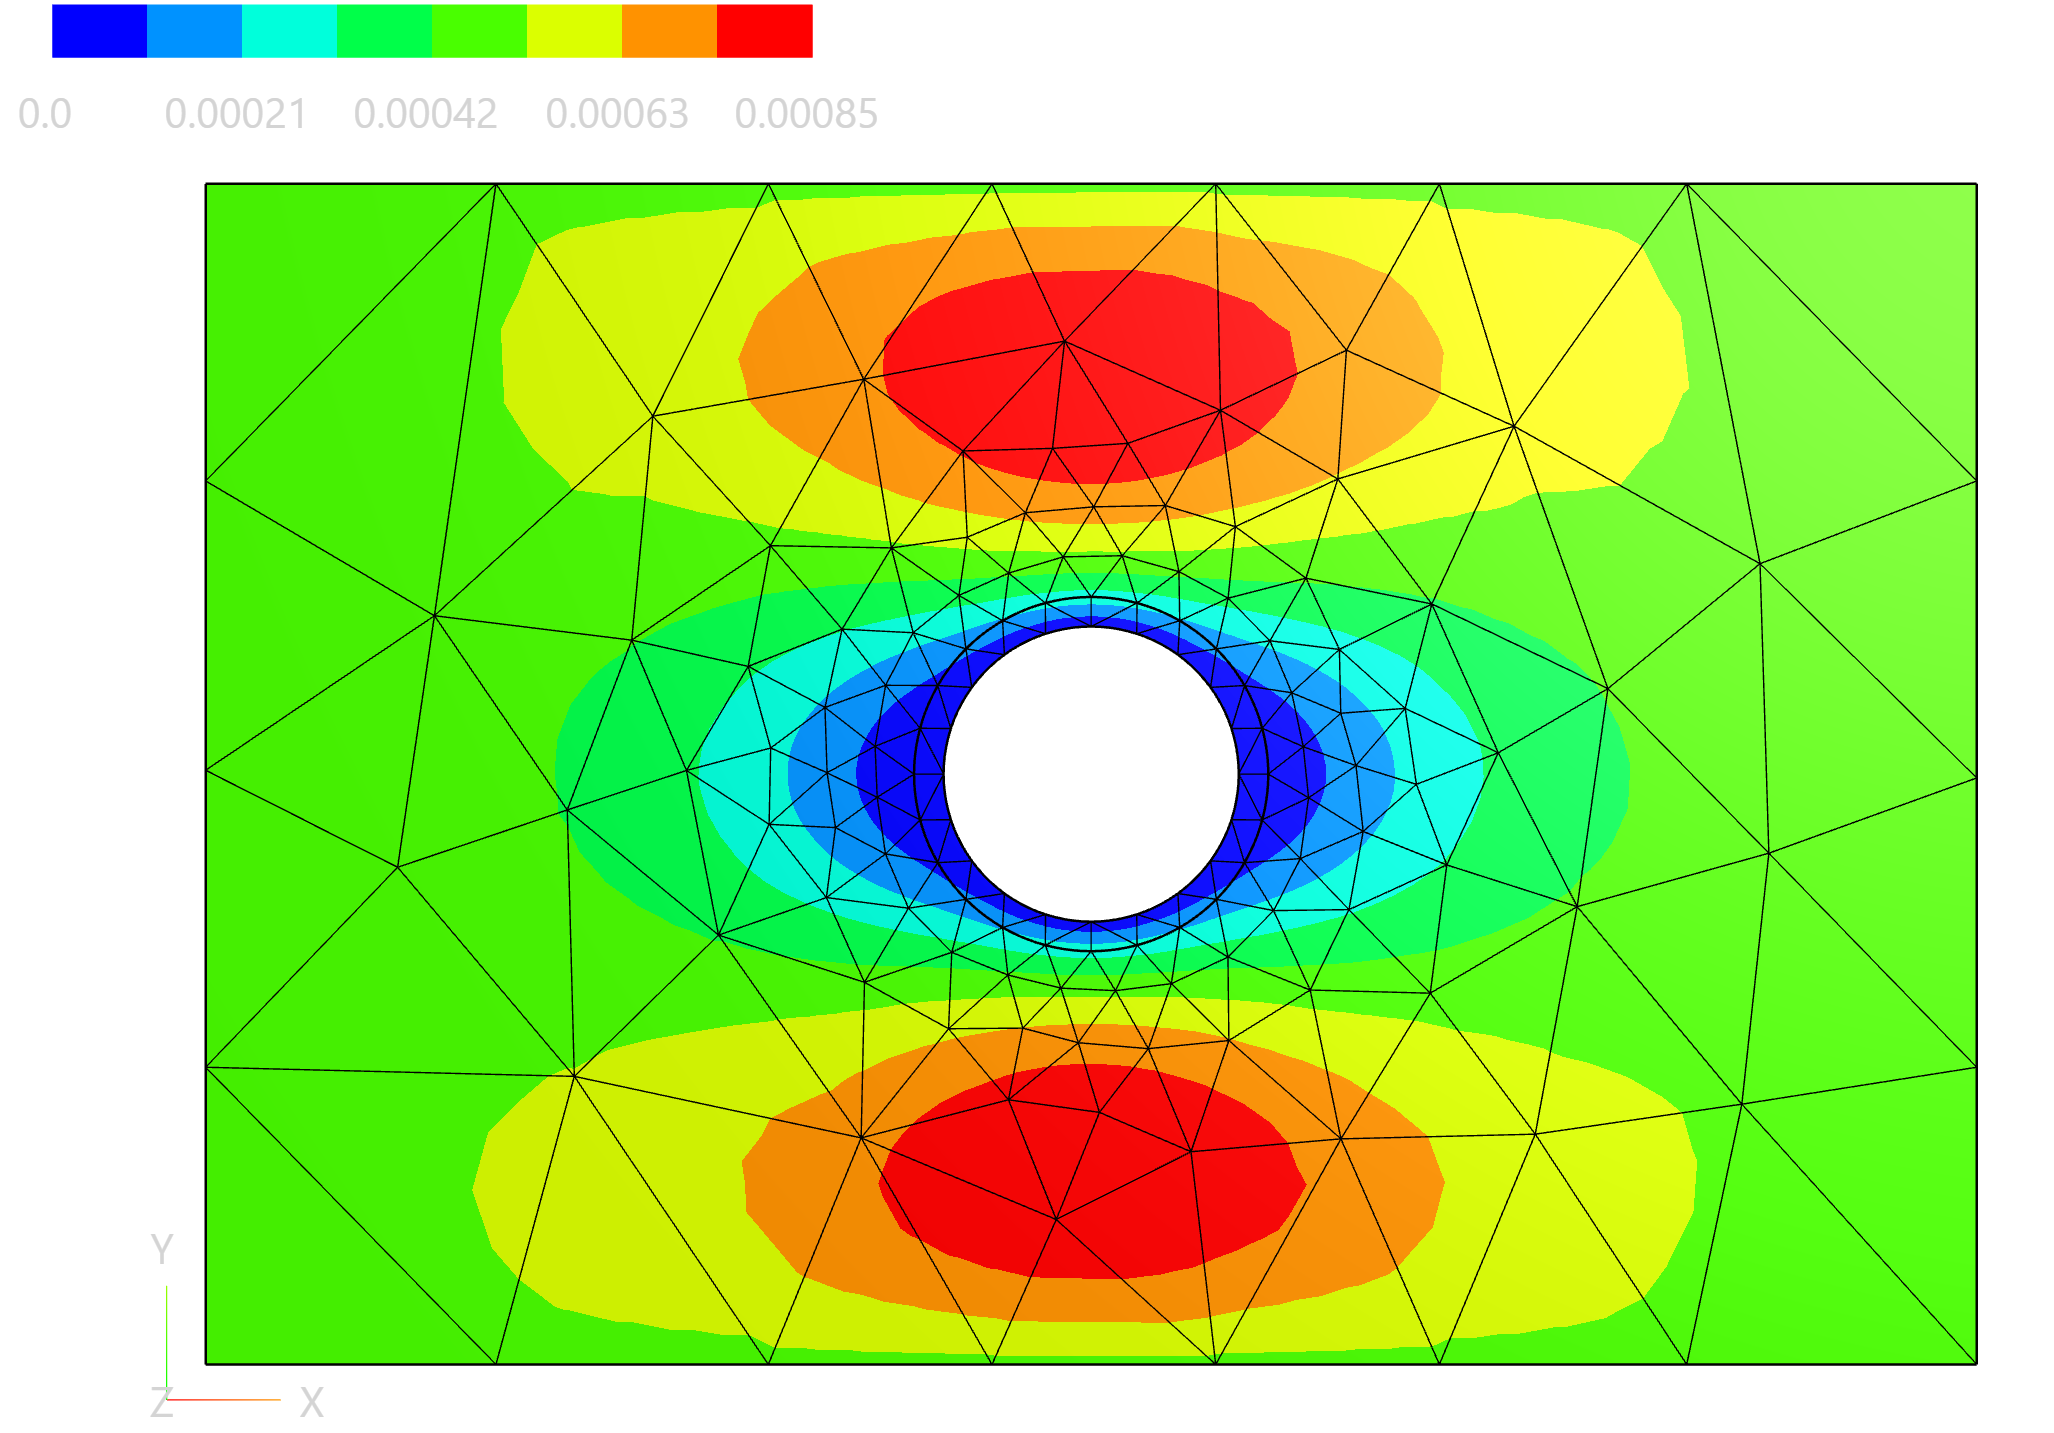
\includegraphics[width=1\textwidth]{figures/u_0.PNG}
    \caption{ $\mathbf{||u||_2}$ on $\Omega_{\mathrm{n}}$ for $\mathrm{n}=0$}
    \label{plot_ref_u_0}
\end{minipage}
\begin{minipage}{.5\textwidth}
    \centering
    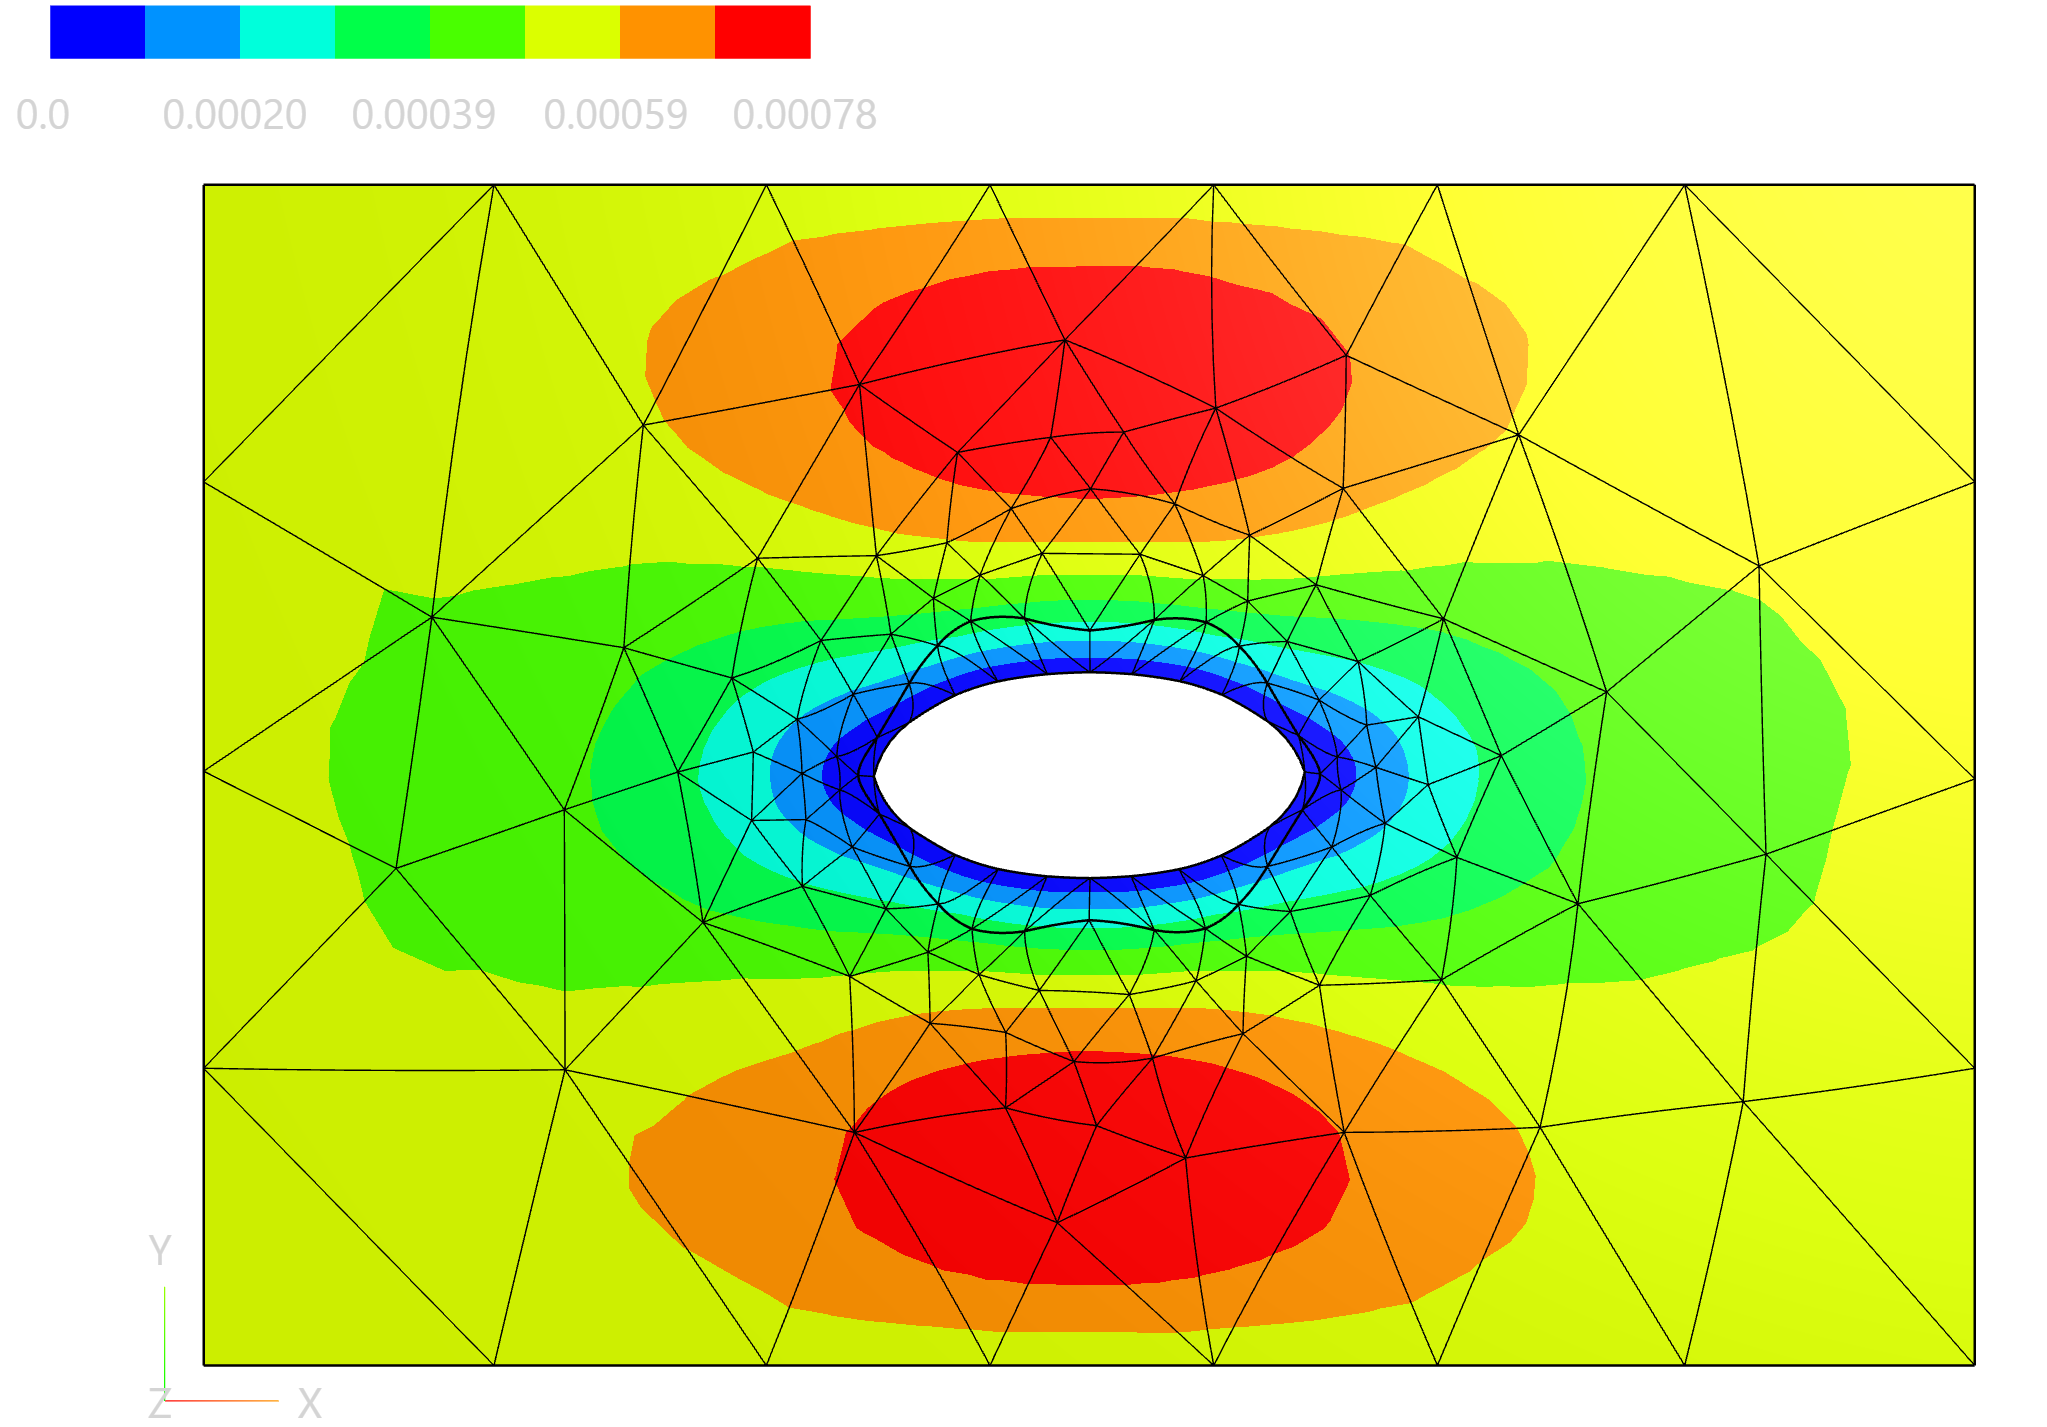
\includegraphics[width=1\textwidth]{figures/u_final.PNG}
    \caption{ $\mathbf{||u||_2}$ on $\Omega_{\mathrm{n}}$ for $\mathrm{n}=800$}
    \label{plot_ref_u_final}
\end{minipage}
\end{figure}

In the figures \ref{plot_ref_u_0} and \ref{plot_ref_u_final} above, the initial and final domains $\Omega$ 
show good agreement with the results obtained by Sturm et. al. \cite{fully_semi_paper_sturm} where the 
tips of the ogive show approximately 45 degree angles. The constraint for near conformality posed in equation
(\ref{eq_conf_aux}) also yields acceptable mesh quality at the tips, where the mesh withouth these contraints
would result in a self intersecting mesh. This renders the Stokes solution $(\mathbf{u},p)$ useless locally.

\begin{figure}[h]
    \begin{center}
        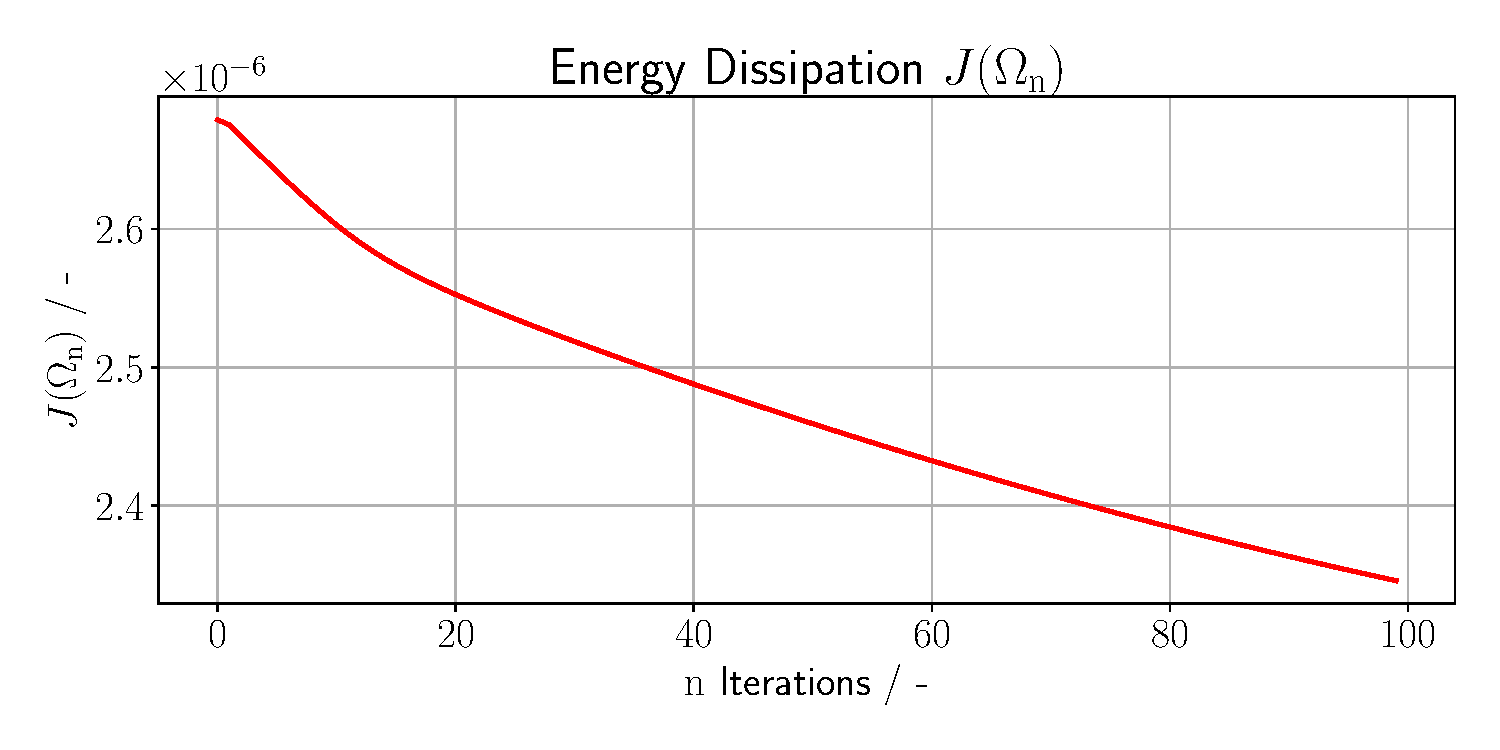
\includegraphics[width=1\textwidth]{figures/energy_diss_plot.pdf}
        \caption{Evaluation of Energy Dissipation on $\Omega$}
        \label{plot_ref_energy_diss}
    \end{center}
\end{figure}

In figure \ref{plot_ref_energy_diss}, convergence of the minimization problem can be observed. However, not
only convergence with respect tho the energy minimization is relevant in the posed problem. Since the 
Augmented Lagrangian (\ref{final_aug_lagrange}) also tracks the quantities $\mathrm{vol}(\Omega_{\mathrm{n}}), \,
\mathrm{\mathrm{bc}_x(\Omega_{\mathrm{n}})}, \, \mathrm{bc}_y(\Omega_{\mathrm{n}})$ by keeping them constant or rather penalize
deviations from the initial value, investigation of these values are also done subsequently.

\pagebreak
\begin{figure}
    \begin{center}
        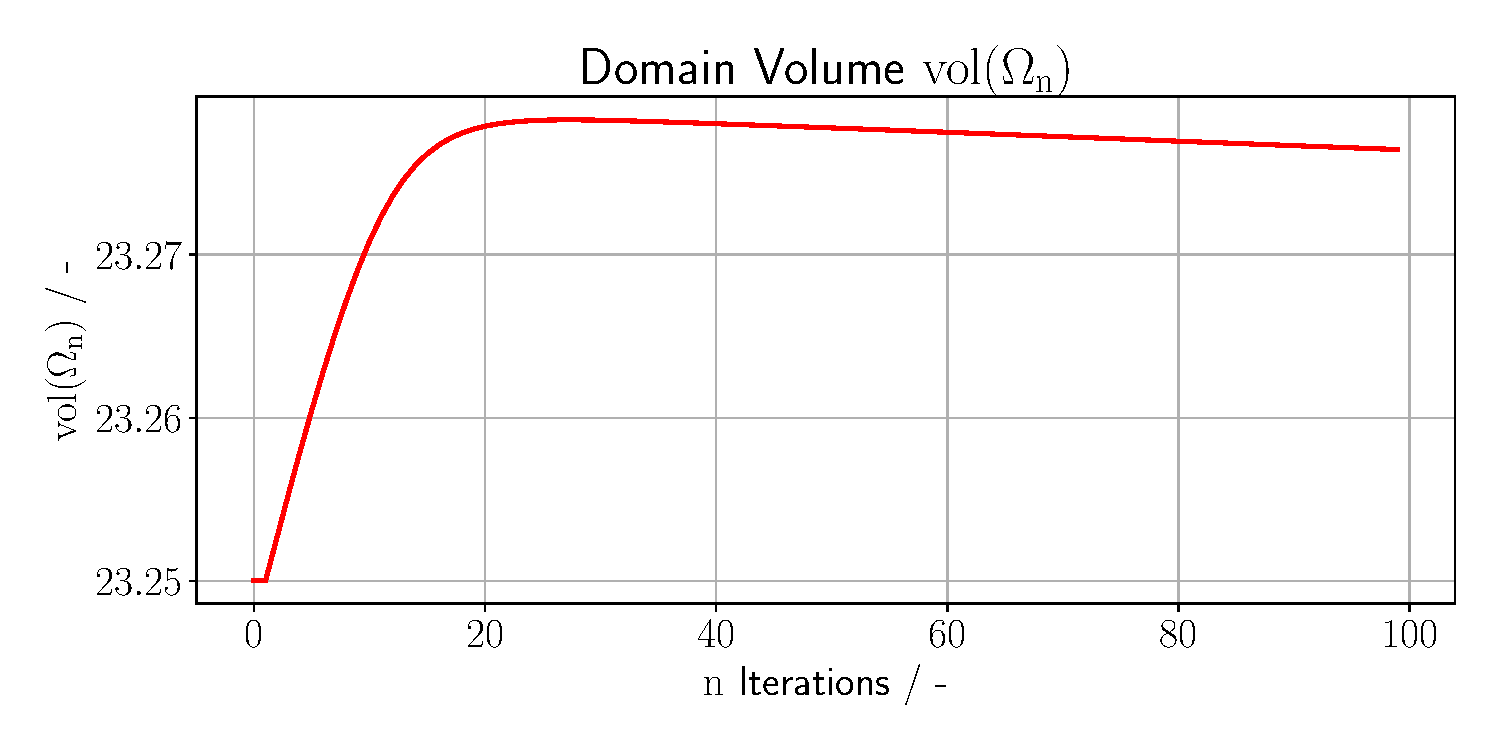
\includegraphics[width=0.8\textwidth]{figures/volume_plot.pdf}
        \caption{Volume of $\Omega$}
        \label{plot_ref_volume}
    \end{center}
\end{figure}
\begin{figure}
    \begin{minipage}{.5\textwidth}
        \centering
        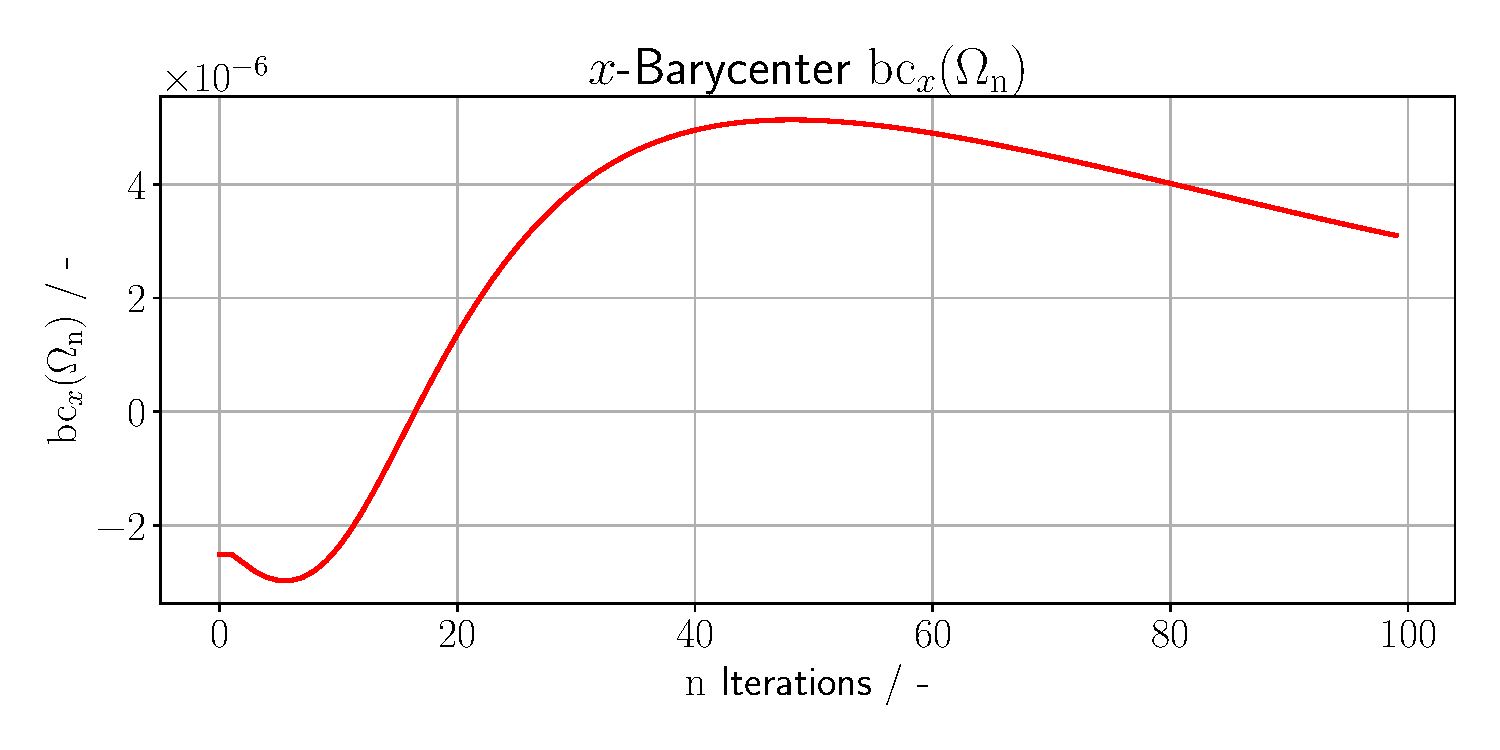
\includegraphics[width=1\textwidth]{figures/bc_x__plot.pdf}
        \caption{$x$ Component of Barycenter of $\Omega$}
        \label{plot_ref_bc_x}
    \end{minipage}
    \begin{minipage}{.5\textwidth}
        \centering
        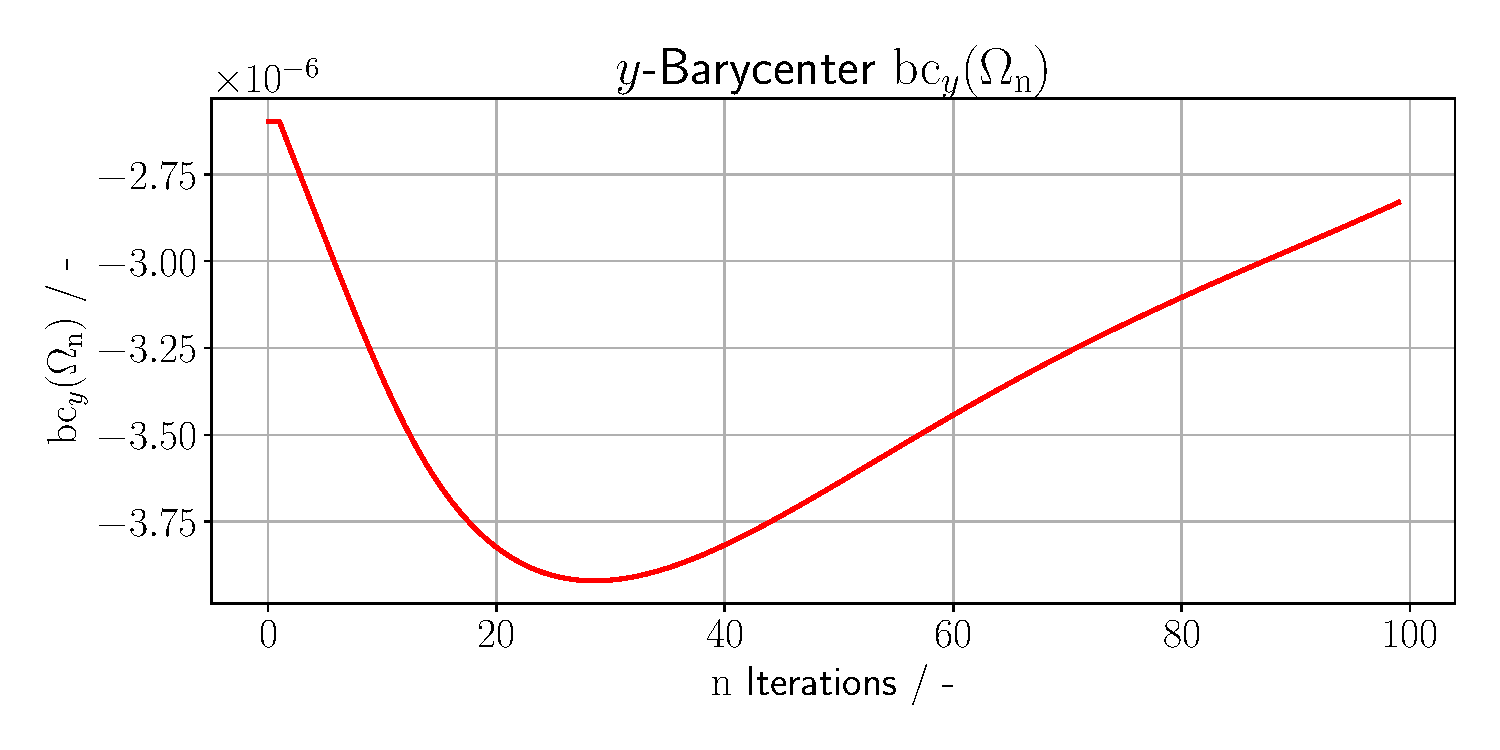
\includegraphics[width=1\textwidth]{figures/bc_y_plot.pdf}
        \caption{$y$ Component of Barycenter of $\Omega$}
        \label{plot_ref_bc_y}
    \end{minipage}
    \end{figure}

In figure \ref{plot_ref_volume}, oscillations around the initial value $\mathrm{vol}(\Omega_0)$ can be
be observed, which further underlines the approximative character of the Augmented Lagrangian Method
(\ref{final_aug_lagrange}). The same behaviour can be observed for the barycenters in $x$ and $y$
directions, which for a symmetric domain $\Omega$ with respects to the coordinate system should
both be 0.
\begin{figure}[h]
    \begin{minipage}{.5\textwidth}
        \centering
        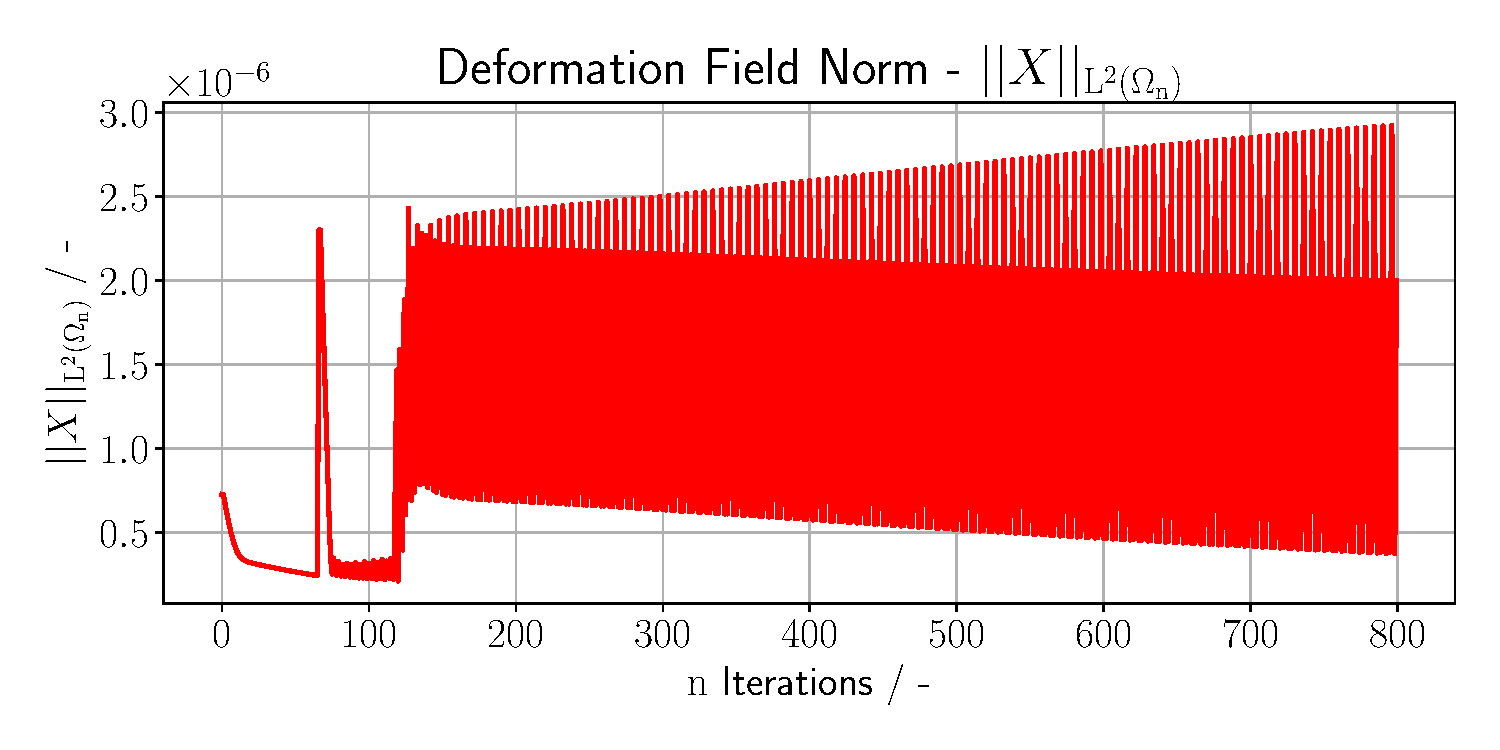
\includegraphics[width=1\textwidth]{figures/gfxnorm_plot.pdf}
        \caption{Norm of $X$ on Domain}
        \label{plot_ref_norm}
    \end{minipage}
    \begin{minipage}{.5\textwidth}
        \centering
        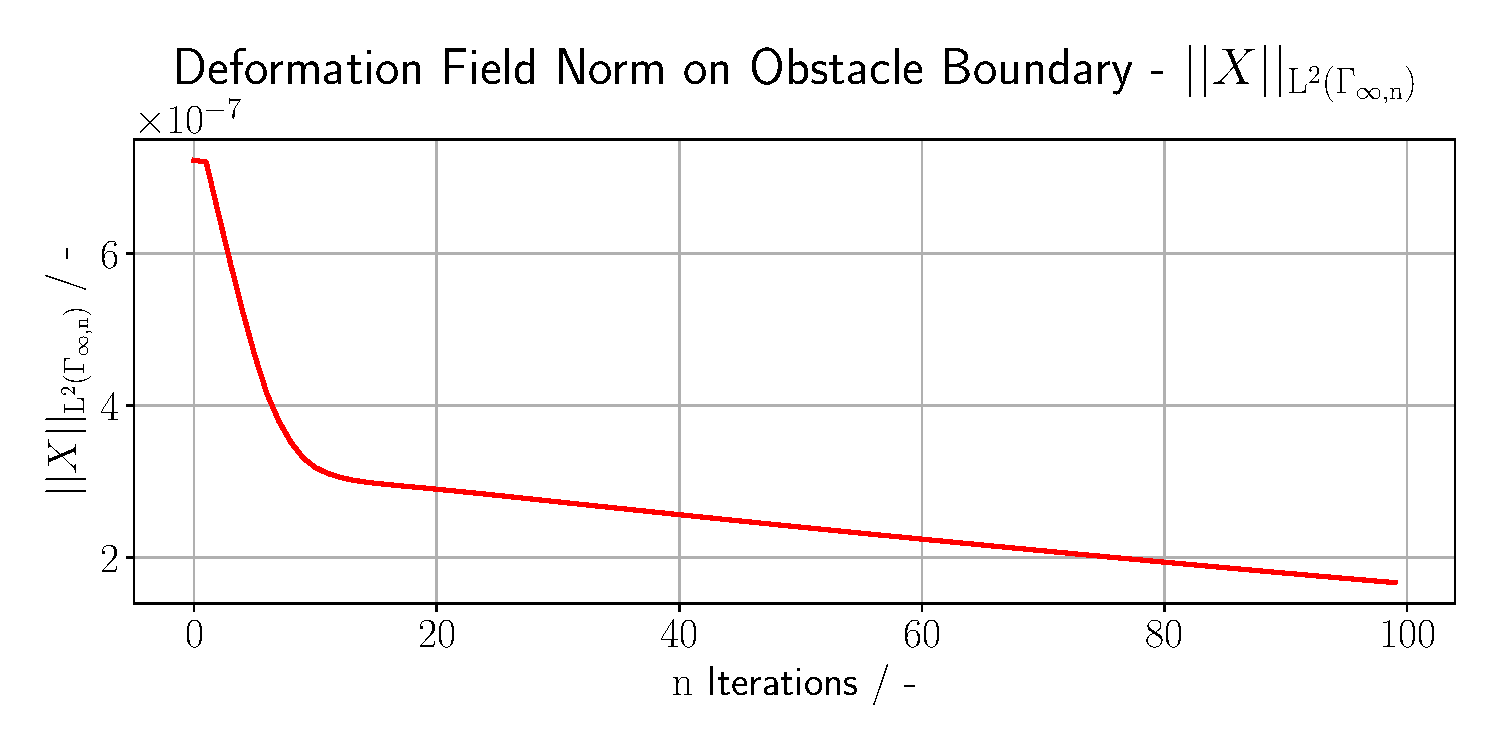
\includegraphics[width=1\textwidth]{figures/gfx_bndnorm_plot.pdf}
        \caption{Norm of $X$ on Boundary}
        \label{plot_ref_bndnorm}
    \end{minipage}
\end{figure}

In figures \ref{plot_ref_norm} and \ref{plot_ref_bndnorm} the $L^2$ norms on the domain
and the obstacle boundary are evaluated. These quantities have similar shape but a scaling factor of 2 
in between. In a subsequent Seminary Project, one could investigate their scaling impact for the iterations
further.

\pagebreak

\subsection{Cauchy-Riemann Constraint Impact on Mesh and Shape}

\begin{figure}[h]
    \begin{minipage}{.5\textwidth}
        \centering
        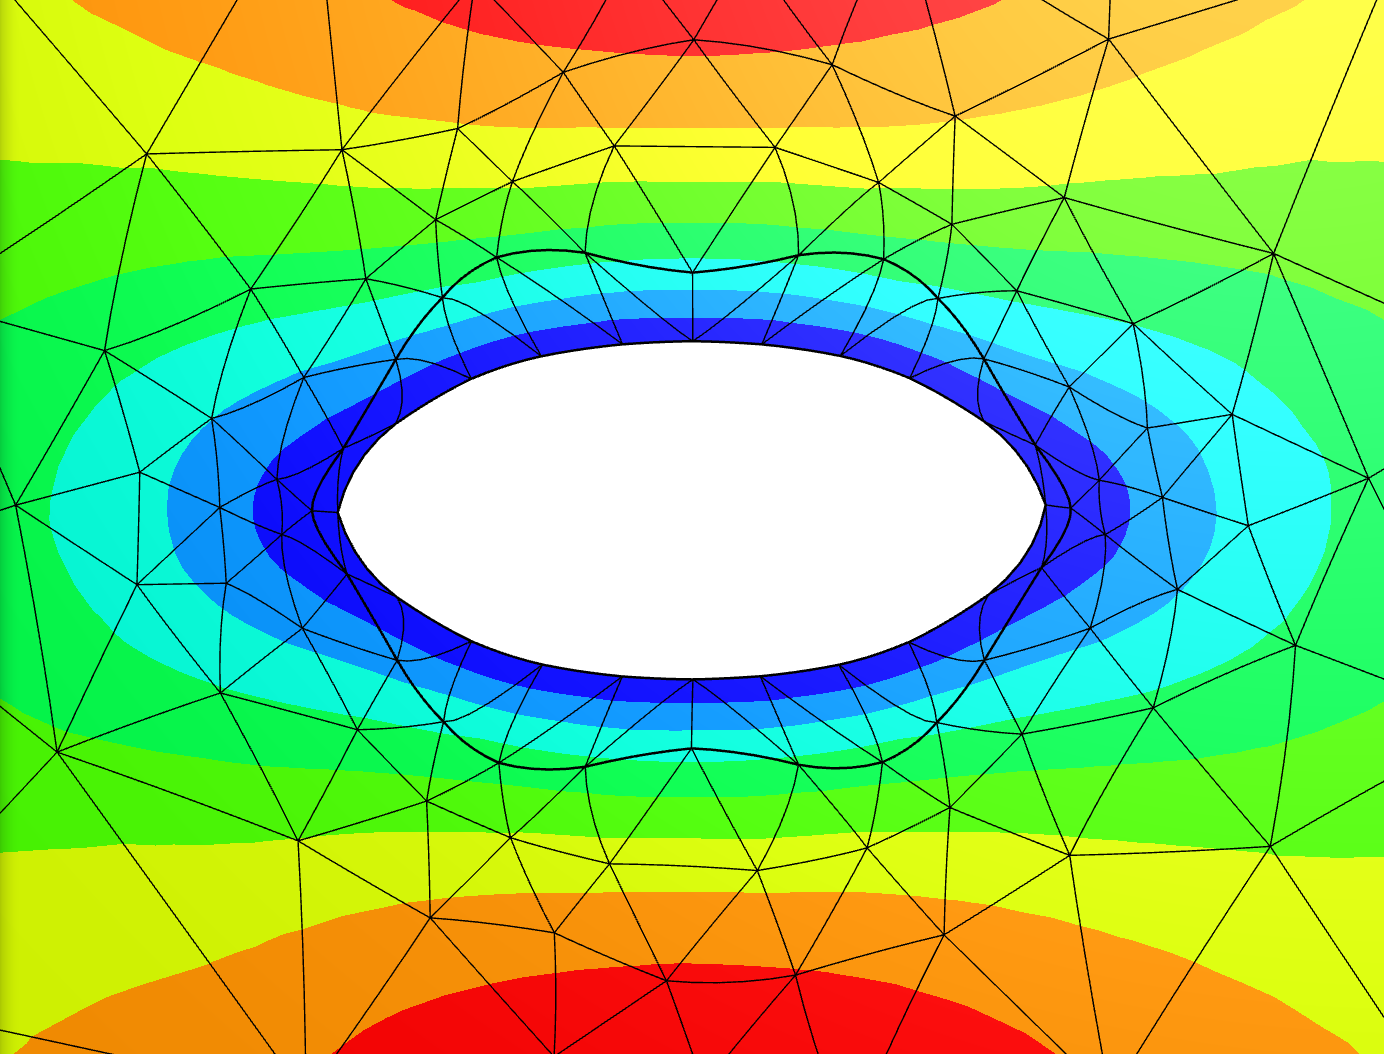
\includegraphics[width=0.97\textwidth]{figures/mesh_good.PNG}
        \caption{Final $\Omega$ with CR Constraint}
        \label{plot_ref_good_mesh_u}
    \end{minipage}
    \begin{minipage}{.5\textwidth}
        \centering
        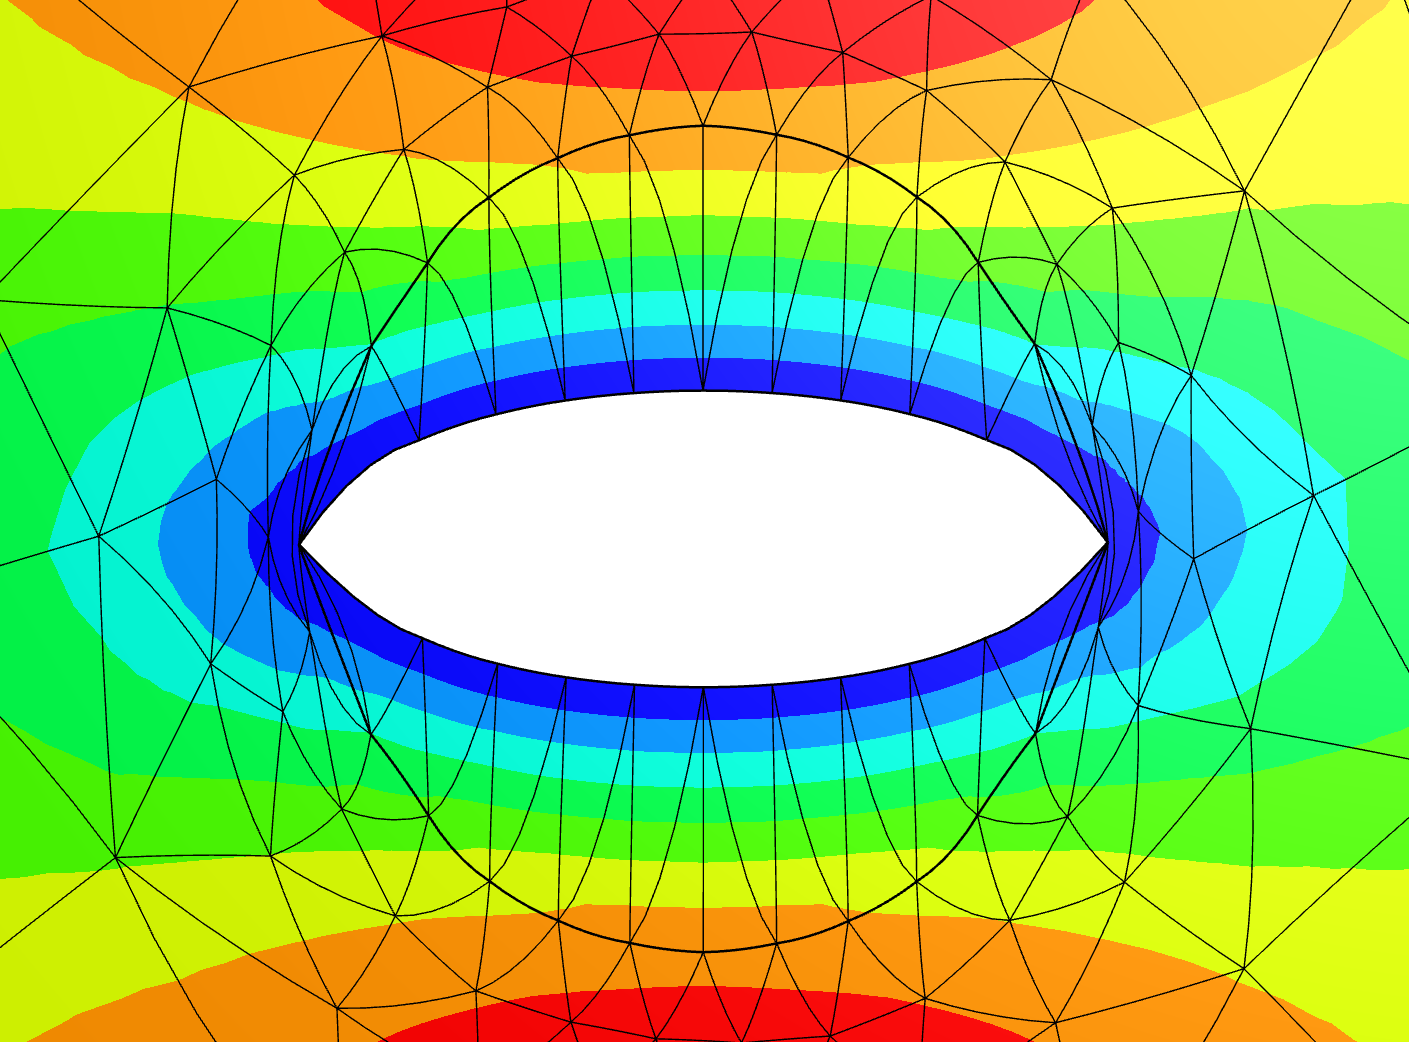
\includegraphics[width=1\textwidth]{figures/mesh_bad.PNG}
        \caption{Final $\Omega$ without CR Constraint}
        \label{plot_ref_bad_mesh_u}
    \end{minipage}
\end{figure}
\begin{figure}[h]
    \begin{minipage}{.5\textwidth}
        \centering
        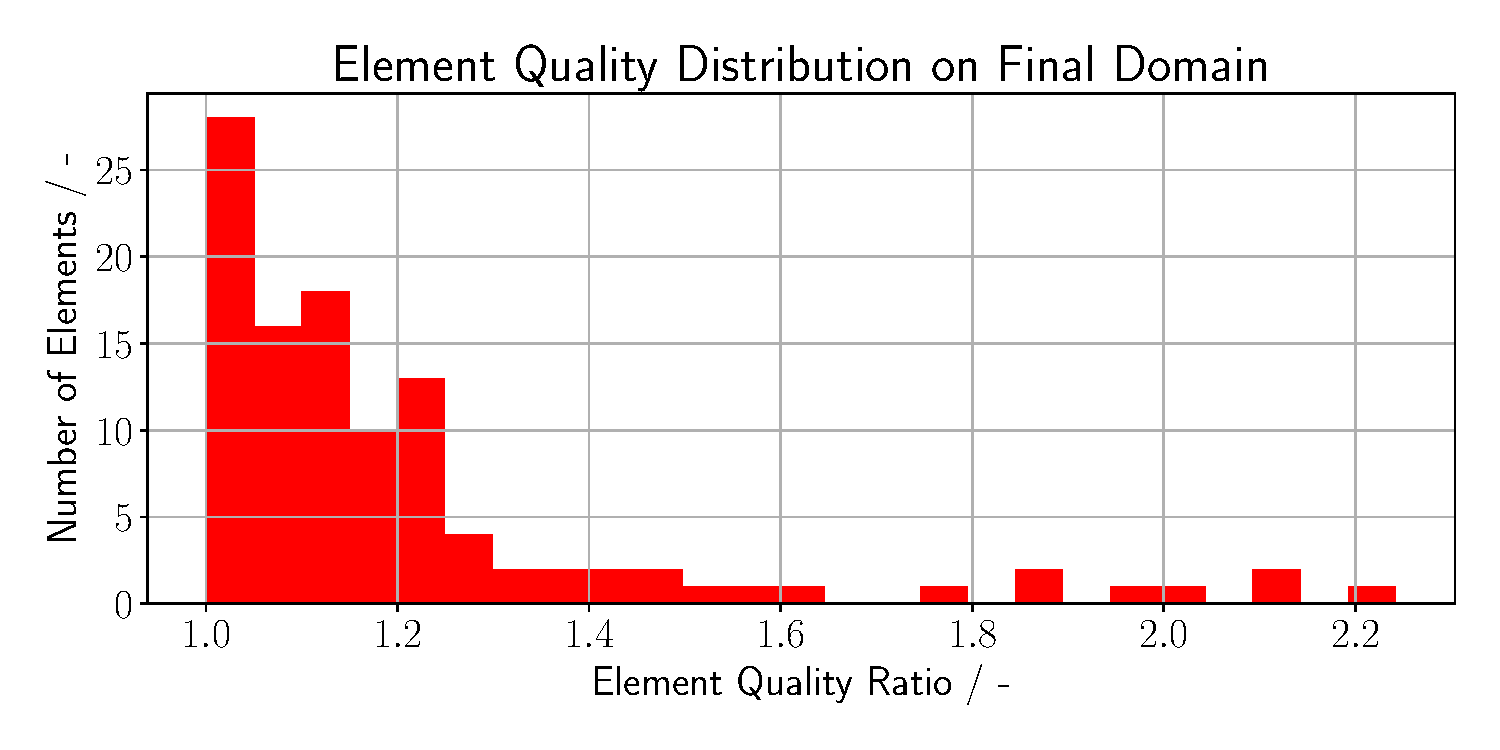
\includegraphics[width=1\textwidth]{figures/element_quality_hist.pdf}
        \caption{Element Quality with CR Constraint}
        \label{plot_ref_element_good}
    \end{minipage}
    \begin{minipage}{.5\textwidth}
        \centering
        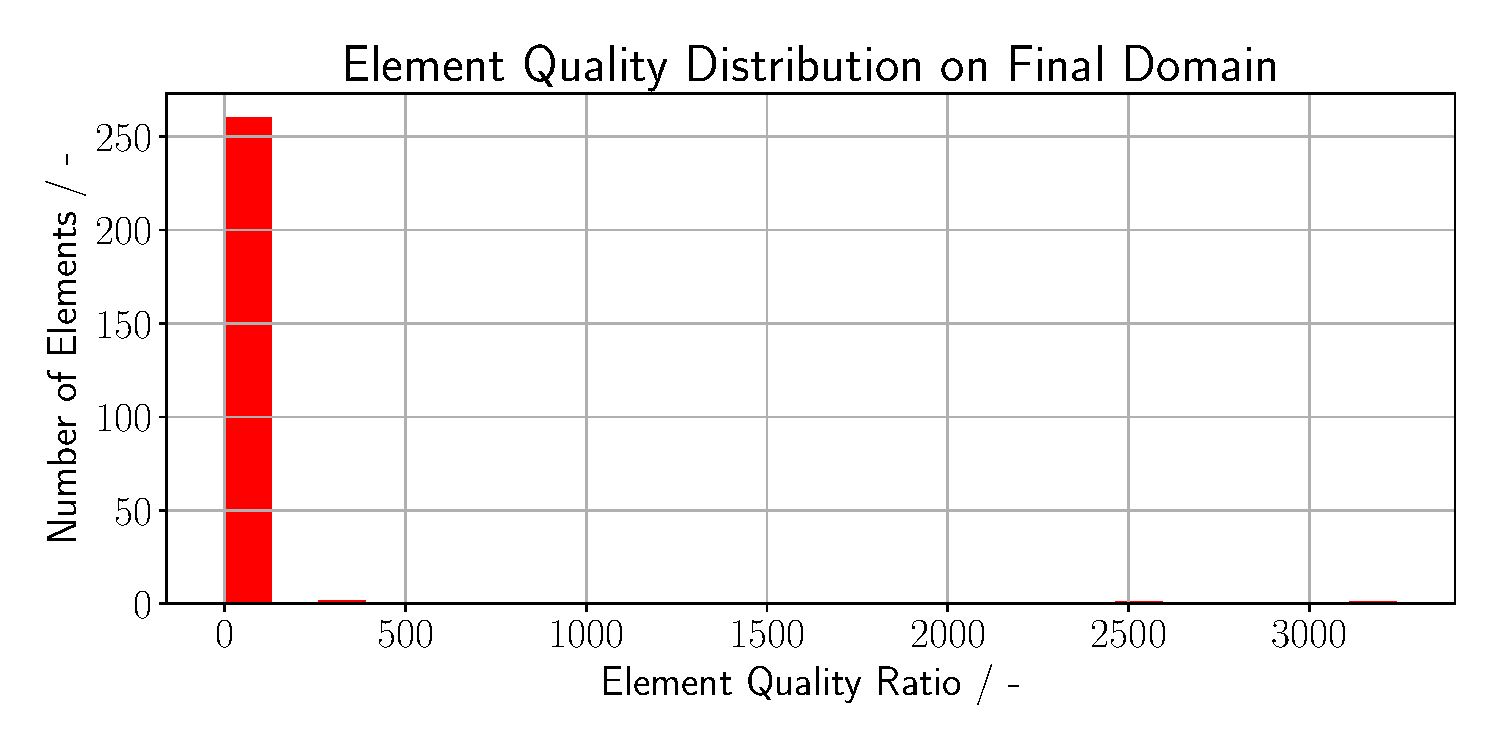
\includegraphics[width=1\textwidth]{figures/element_quality_hist_bad.pdf}
        \caption{Element Quality without CR Constraint}
        \label{plot_ref_element_bad}
    \end{minipage}
\end{figure}

In figures \ref{plot_ref_good_mesh_u} - \ref{plot_ref_element_bad}, the impact of the Cauchy-Riemann 
constraint can be observed. The mesh in figure \ref{plot_ref_bad_mesh_u} adjacent to the obstacle is
highly distorted and the solutions $(\mathbf{u},p)$ therefore not reliable anymore. The element quality 
at the tips is approximately 3000 without the CR constraint, as shown in figure \ref{plot_ref_element_bad}.
With applied CR constraint with $\alpha = 150$, the minimization after 800 iterations results in a acceptable
element quality distribution, as shown in figures \ref{plot_ref_good_mesh_u} and \ref{plot_ref_element_good}.

\pagebreak

\subsection{Cauchy-Riemann Constraint Impact on Convergence Behaviour}
\begin{figure}[h]
    \begin{minipage}{.5\textwidth}
        \centering
        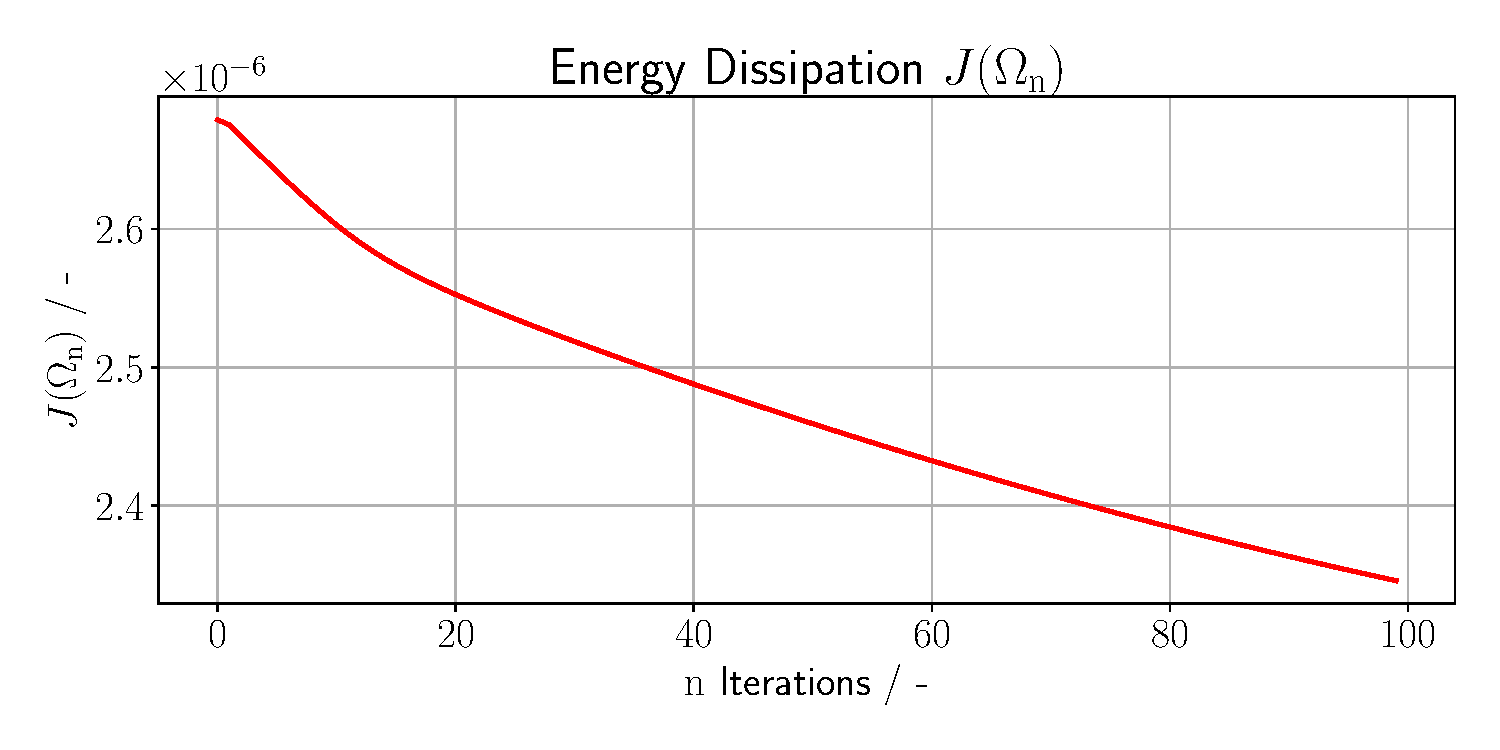
\includegraphics[width=1\textwidth]{figures/energy_diss_plot.pdf}
        \caption{Energy Diss. with CR Constraint}
        \label{plot_ref_energy_diss_good}
    \end{minipage}
    \begin{minipage}{.5\textwidth}
        \centering
        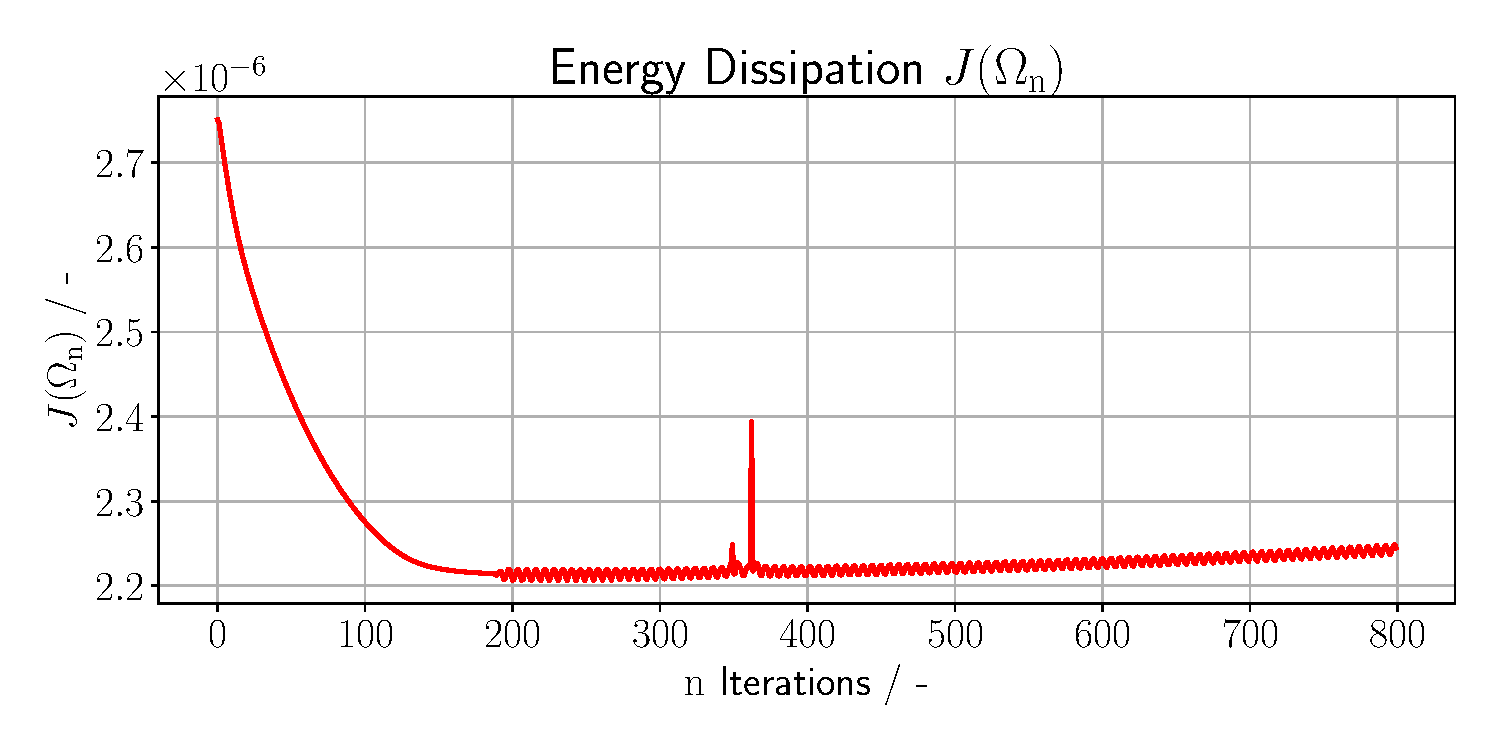
\includegraphics[width=1\textwidth]{figures/energy_diss_plot_bad.pdf}
        \caption{Energy Diss. without CR Constraint}
        \label{plot_ref_energy_diss_bad}
    \end{minipage}
\end{figure}
\begin{figure}[h]
    \begin{minipage}{.5\textwidth}
        \centering
        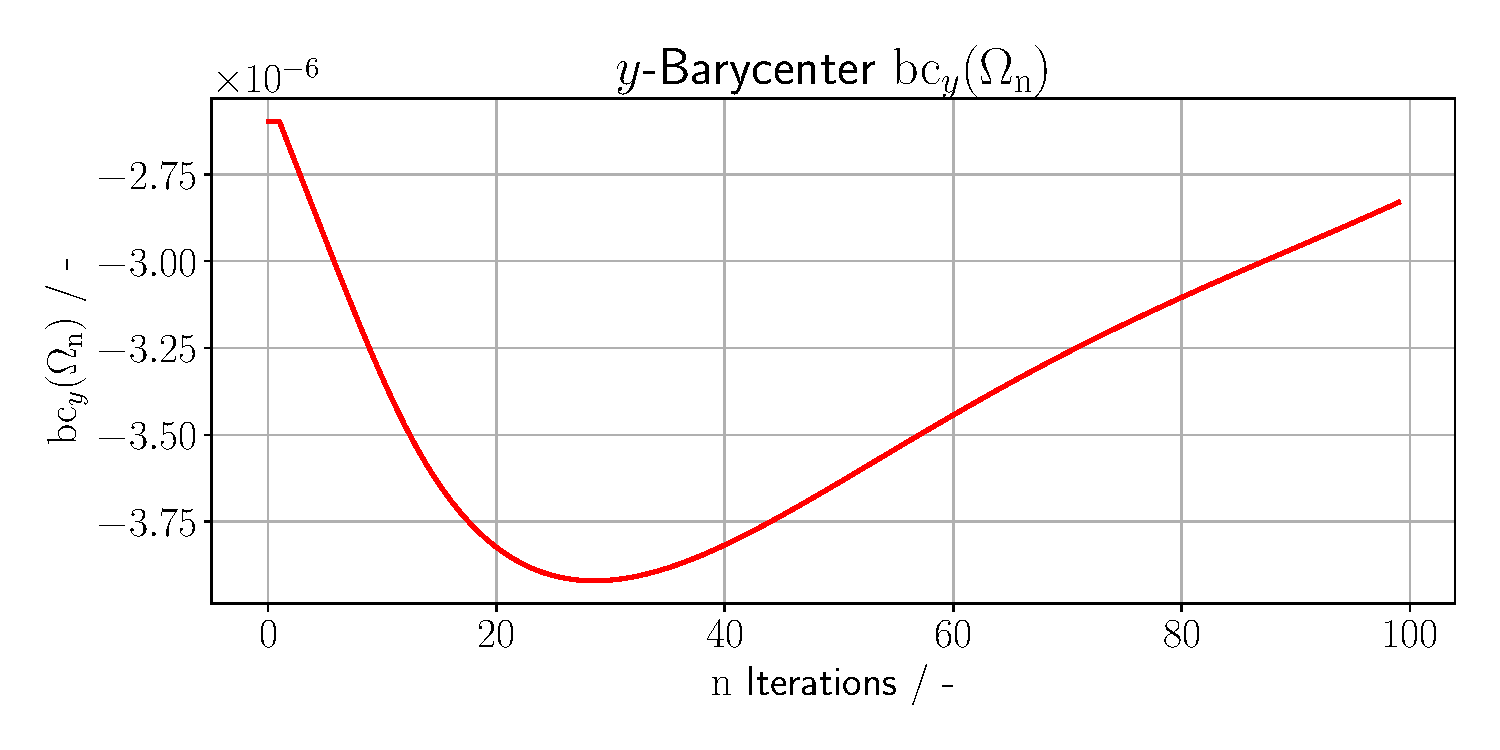
\includegraphics[width=1\textwidth]{figures/bc_y_plot.pdf}
        \caption{$y$-Barycenter with CR Constraint}
        \label{plot_ref_bc_y_good}
    \end{minipage}
    \begin{minipage}{.5\textwidth}
        \centering
        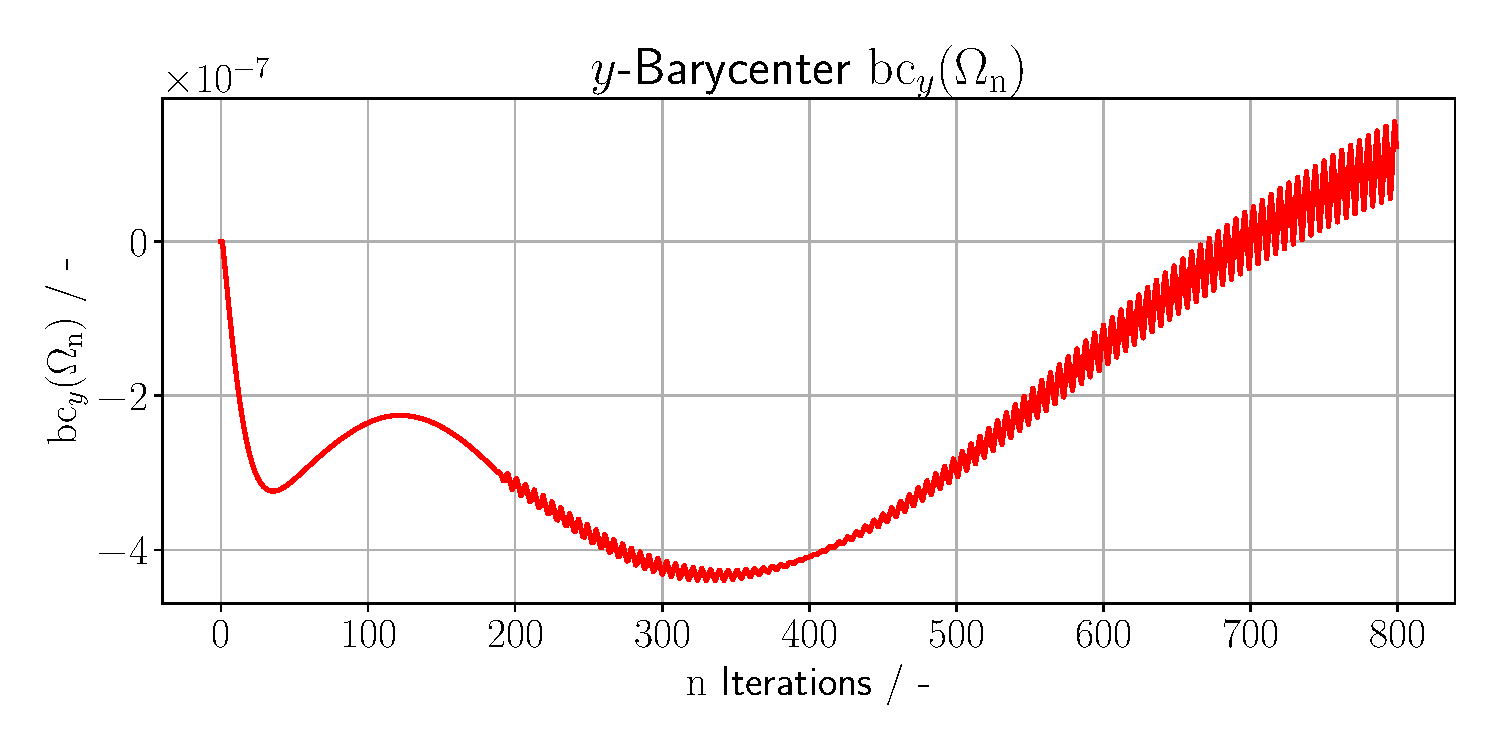
\includegraphics[width=1\textwidth]{figures/bc_y_plot_bad.pdf}
        \caption{$y$-Barycenter without CR Constraint}
        \label{plot_ref_bc_y_bad}
    \end{minipage}
\end{figure}
\begin{figure}[h]
    \begin{minipage}{.5\textwidth}
        \centering
        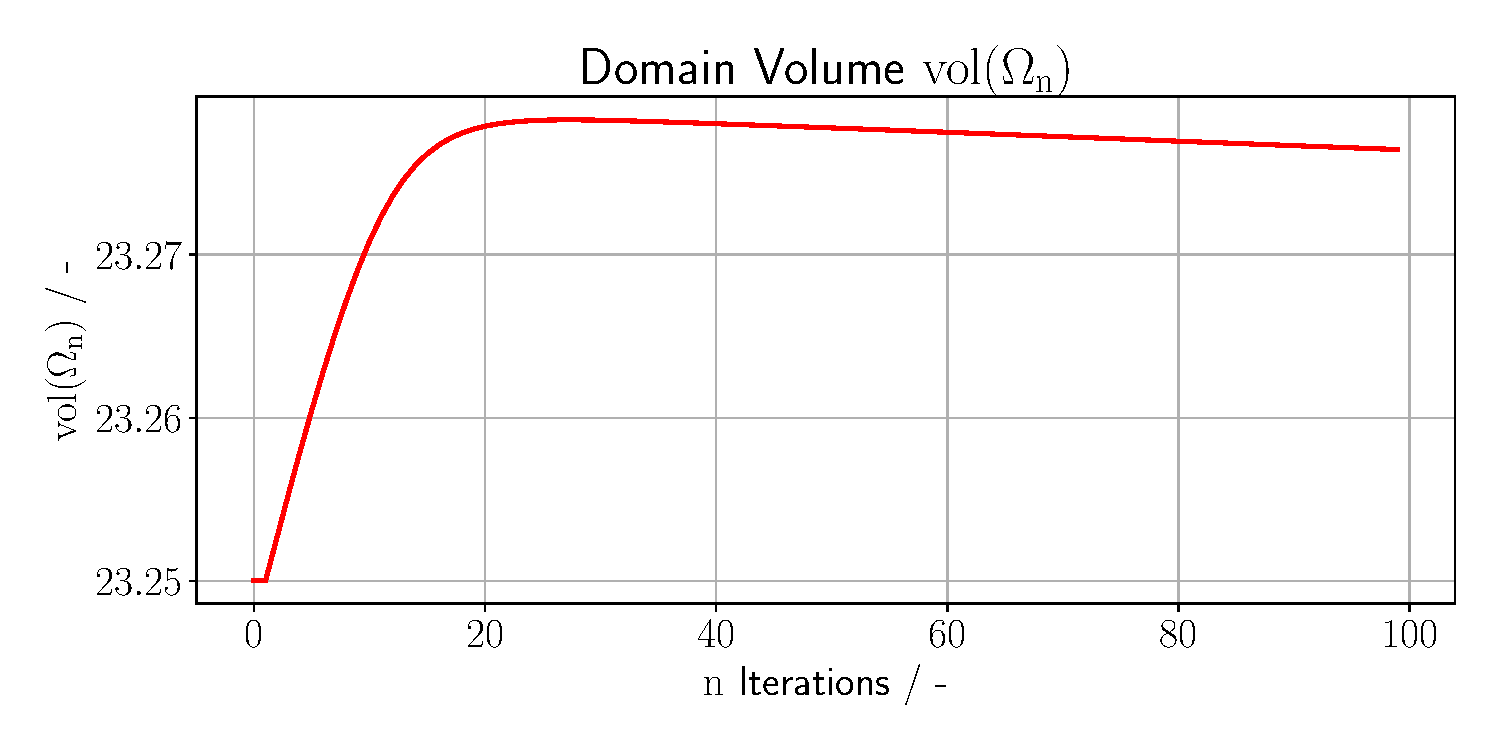
\includegraphics[width=1\textwidth]{figures/volume_plot.pdf}
        \caption{Volume with CR Constraint}
        \label{plot_ref_vol_good}
    \end{minipage}
    \begin{minipage}{.5\textwidth}
        \centering
        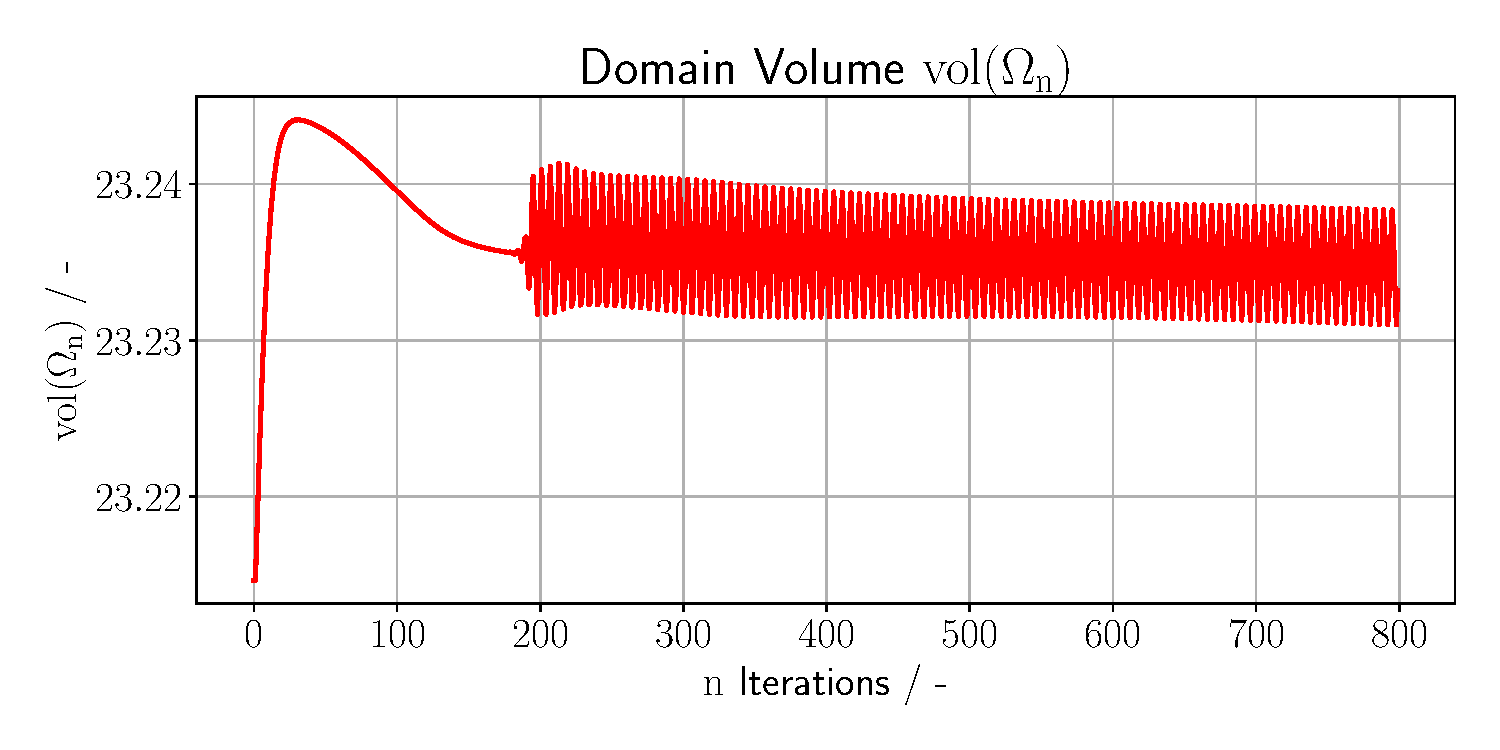
\includegraphics[width=1\textwidth]{figures/volume_plot_bad.pdf}
        \caption{Volume wihtout CR Constraint}
        \label{plot_ref_vol_bad}
    \end{minipage}
\end{figure}

In figure \ref{plot_ref_energy_diss_bad}, the energy dissipation increases again after 200 iterations,
while the $y$-barycenter in figure \ref{plot_ref_bc_y_bad} and the volume of $\Omega$ 
Figure \ref{plot_ref_vol_bad} are not nearly in the vicinity of the desired initial values.
For this PDE-Constrained Shape optimization setup, the CR-Equations are therefore even needed,
since no convergence can be observed without them for all tracked quantities.

\pagebreak